%%%%%%%%%%%%%%%%%%%%%%%%%%%%%%%%%%%%%%%%%%%%%%%%%%%%%%%%%%%%%%%%
\subsection{PK with Poisson model}
\label{subsec:PKPDcount}

%%%%%%%%%%%%%%%%%%%%%%%%%%%%%%%%%%%%%%%%%%%%%%%%%%%%%%%%%%%%%%%%
\paragraph{Introduction}

The key element of this task is the probability distribution of count data \emph{y}, which can be defined as either $P(y=k)$ or $\log(P(y=k))$ or $logit(P(y=k))$. In this example, $k \in {1,2, .., n}$. The underlying PK model is 1-compartmental oral model. Then we estimate the log-likelihood that the outcome is $k$ using the non-homogeneous Poisson model 
\begin{eqnarray}
&& P\big(y_{ij}=k | Cc_{ij}, \psi_i\big) =  \frac{e^{-\lambda_{ij}} \lambda^k_{ij}}{k!} \nonumber
\end{eqnarray}
with concentration dependent mean $\lambda$
\begin{eqnarray}
&& \lambda_{ij} = \lambda0 \Big(1 - \frac{Cc_{ij}}{IC50 + Cc_{ij}}\Big)  \nonumber
\end{eqnarray}
also called Poisson intensity. Here, $\lambda$, depends on the parameters $\lambda0$ and $IC50$ which are sampled from log-normal distribution. $\lambda0$, stands here for the baseline seizure count prior to any drug. The value of $\lambda$ is reduced by the concentration in the central compartment, $Cc$, which is visualised for three different values of $Cc = \{1,5,15\}$ in \ref{fig:lambdasurface} ($1\equiv$ green, $5 \equiv$ red, $15 \equiv$ blue).

\begin{figure}[htbp]
\centering
\begin{tabular}{cc}
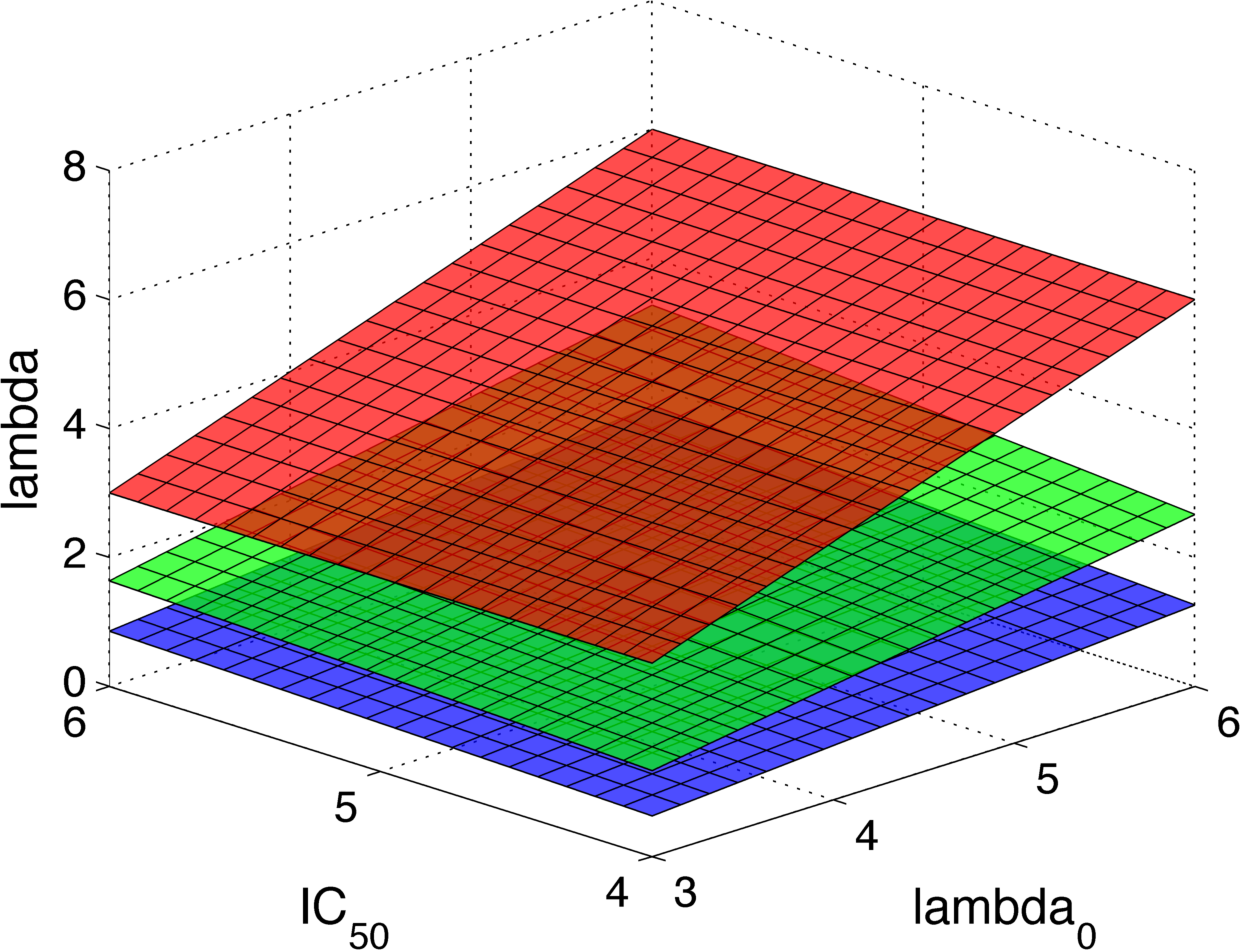
\includegraphics[width=.45\textwidth]{pics/CTS4_lambda_threeSurfaces} & 
\raisebox{0\height}{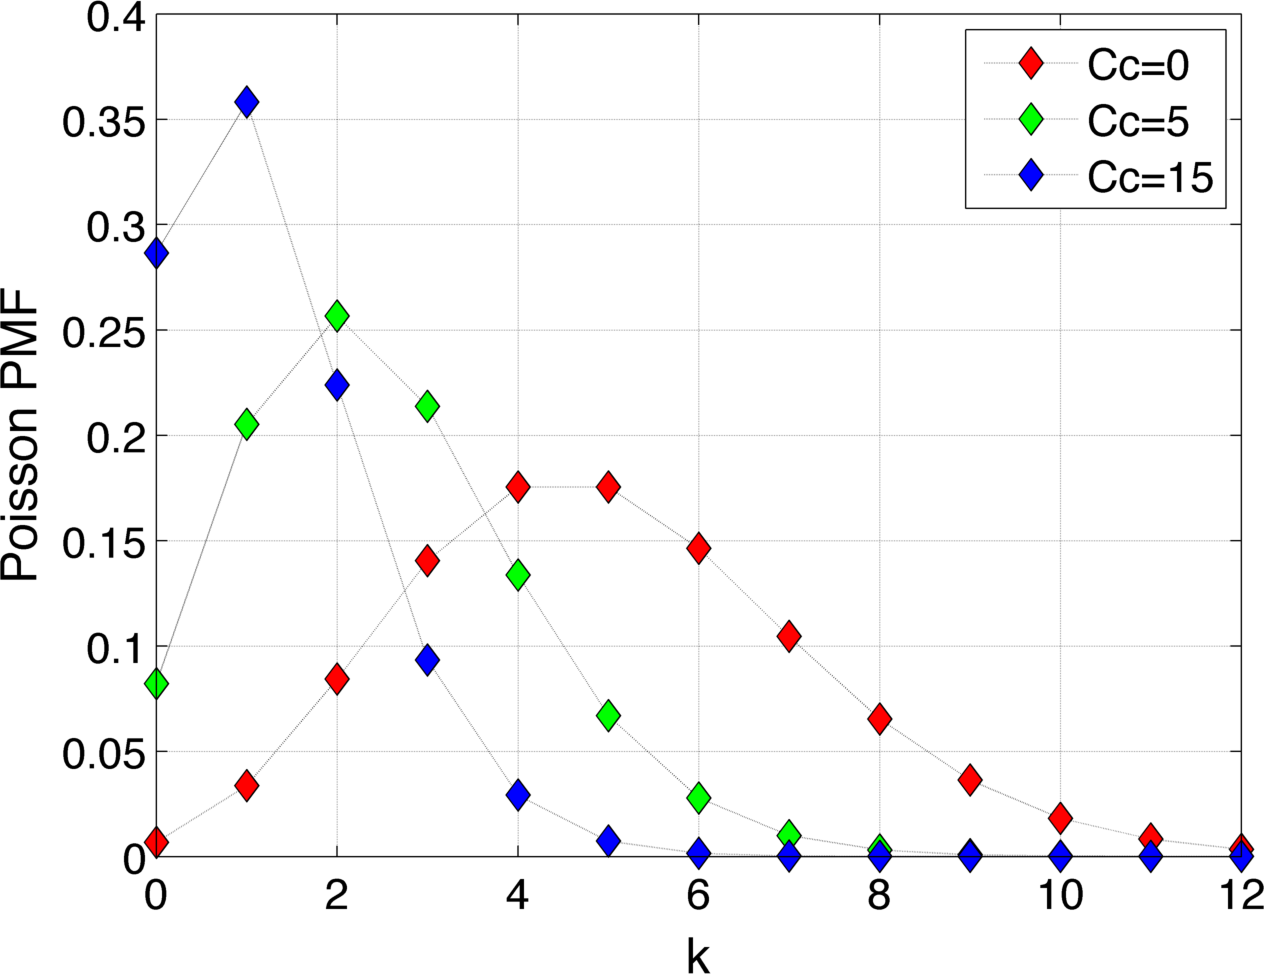
\includegraphics[scale=0.45]{pics/CTS4_poissonScan}}
\end{tabular}
\caption{(LEFT) $\lambda$--surface as function of $\lambda0$ and $IC50$ plotted for $Cc = \{1,5,15\}$. (RIGHT) Poisson PMF for fixed parameters $\lambda0 = IC50 = 5$ and varying concentration $Cc = \{1,5,15\}$.}
\label{fig:lambdasurface}
\end{figure}


%%%%%%%%%%%%%%%%%%%%%%%%%%%%%%%%%%%%%%%%%%%%%%%%%%%%%%%%%%%%%%%%
\subsubsection{Model description}
\label{subsec:exp5_TaskDescription}

%\paragraph{Individual parameters model}
%
%Details omitted here...
%
%\begin{eqnarray}
%ka& \sim& \mbox{logNormal}(ka_{\rm pop}, \omega_{ka});  \quad ka_{\rm pop}=1,\quad \omega_{ka}=0.6 \nonumber \\
%V& \sim& \mbox{logNormal}(V_{\rm pop}, \omega_{V}); \quad V_{\rm pop}=8,\quad \omega_V=0.2 \nonumber \\
%CL& \sim&  \mbox{logNormal}(CL_{\rm pop}, \omega_{CL}); \quad CL_{\rm pop}=0.13,\quad \omega_{CL}=0.2 \nonumber \\
%\lambda0 & \sim&  \mbox{logNormal}(\lambda0_{{\rm pop}}, \omega_{\lambda0}); \quad  \lambda0_{{\rm pop}} = 5, \quad \omega_{\lambda0} = 0.2 \nonumber \\
%IC50 &\sim& \mbox{logNormal}(IC50_{{\rm pop}}, \omega_{IC50}); \quad  IC50_{{\rm pop}} = 5, \quad \omega_{IC50} = 0 \nonumber
%\end{eqnarray}
%\begin{eqnarray}
%\log(V_i) &=& \log(V_{pop}) + \beta_{1,V}\log(W_i/70) + \eta_{V,i} \nonumber \\
%\log(CL_i) &=& \log(CL_{pop}) + \beta_{1,CL}\log(W_i/70) + \eta_{CL,i} \nonumber \\
%\beta_{1,V}&=&1 \nonumber \\
%\beta_{1,CL}&=&0.75 \nonumber \\
%\rho_{V,CL}&=&0.7 \mbox{  (the correlation coefficient between } \eta_{V,i} \mbox{ and } \eta_{CL,i}  \mbox{)} \nonumber
%\end{eqnarray}


\paragraph{Structural model}
\begin{eqnarray}
\frac{dAd}{dt} &=&-ka \times Ad \nonumber \\
\frac{dAc}{dt}&=&ka \times Ad - k \times Ac \nonumber \\ 
Cc &=& Ac/V \nonumber \\ \nonumber
\end{eqnarray}
\paragraph{Observation model}

\begin{itemize}
\item
Data type: discrete/count 
\item
Count variable: $Y$
\item
log(Poisson PMF)
\begin{align}
& Log(P(Y=k)) = -\lambda + k\times log(\lambda) - \log(k!) \nonumber
\end{align}
\item
Rate parameter $\lambda$, the Poisson 'intensity' is function of drug concentration, $Cc$
\begin{align}
& \lambda = \lambda0 (1 - Cc/(IC50 + Cc)) \nonumber
\end{align}
\end{itemize}

\subsubsection{PharmML code}
The code below covers the Observation model with eqs.(\ref{eq:logPMF}) and (\ref{eq:lambda}).
All parameters are assumed to be defined in the \xelem{ParameterModel}.
\lstset{language=XML}
\begin{lstlisting}
        <ObservationModel blkId="om1">
            <Discrete>
                <CountData>
                    <CountVariable symbId="k"/>
                    
                    <!-- Poisson intensity - function of drug concentration, Cc -->                    
                    <IntensityParameter symbId="Lambda">
                        <ct:Assign>
                            <math:Equation>
                                <math:Binop op="times">
                                    <ct:SymbRef blkIdRef="pm1" symbIdRef="lambda0"/>
                                    <math:Binop op="minus">
                                        <ct:Real>1</ct:Real>
                                        <math:Binop op="divide">
                                            <ct:SymbRef blkIdRef="sm1" symbIdRef="Cc"/>
                                            <math:Binop op="plus">
                                                <ct:SymbRef blkIdRef="pm1" symbIdRef="IC50"/>
                                                <ct:SymbRef blkIdRef="sm1" symbIdRef="Cc"/>
                                            </math:Binop>
                                        </math:Binop>
                                    </math:Binop>
                                </math:Binop>
                            </math:Equation>
                        </ct:Assign>
                    </IntensityParameter>
                    
                    <!-- log(P(Y=k)) = -lambda+k*log(lambda)-log(k!) -->
                    <PMF linkFunction="log">
                        <math:LogicBinop op="eq">
                            <ct:SymbRef symbIdRef="Y"/>
                            <ct:SymbRef symbIdRef="k"/>
                        </math:LogicBinop>
                        <PoissonDistribution xmlns="http://www.uncertml.org/3.0" 
                            definition="http://www.uncertml.org/3.0">
                            <rate>
                                <var varId="Lambda"/>
                            </rate>
                        </PoissonDistribution>
                    </PMF>
                </CountData>
            </Discrete>
        </ObservationModel>
\end{lstlisting}

